\chapter{Detailed information on hand-assembled noise filters used in this thesis}

\section{Low-pass filter PCB components}\label{app:lowpassfilter}

The low-pass filters consist of two-stage RC filters with the following values:
$R_1=\SI{470}{\ohm}$\footnote{Farnell 121-5922 MMU01020C4700FB300 - Surface Mount MELF Resistor, \SI{470}{\ohm}, MMU 0102 Series, \SI{100}{V}, Metal Film, \SI{100}{\milli\watt}, $\pm\SI{1}{\percent}$}, $R_2=\SI{2}{\kilo\ohm}$\footnote{Farnell 171-7632 ERA6ARB202V - SMD Chip Resistor, 0805 [2012 Metric], \SI{2}{\kilo\ohm}, ERA6A Series, \SI{100}{V}, Metal Film, 125 mW}\footnote{Farnell 121-5939 MMU01020C2001FB300 - Surface Mount MELF Resistor, \SI{2}{\kilo\ohm}, MMU 0102 Series, \SI{100}{V}, Metal Film, \SI{200}{\milli\watt}, $\pm\SI{1}{\percent}$ (these are round ones)}, $C_1=\SI{10}{\nano\farad}$\footnote{Farnell 882-0074 GRM2195C1H103JA01D - SMD Multilayer Ceramic Capacitor, \SI{10000}{\pico\farad}, \SI{50}{V}, 0805 [2012 Metric], $\pm\SI{5}{\percent}$, C0G / NP0, GRM Series}, $C_2=\SI{470}{\pico\farad}$\footnote{Farnell 180-0825 C0805C471J2GACTU - SMD Multilayer Ceramic Capacitor, \SI{470}{\pico\farad}, \SI{200}{V}, 0805 [2012 Metric], $\pm\SI{5}{\percent}$, C0G / NP0}

The connectors for the filter PCBs can also be bought on Farnell\footnote{134-2652 19-70-1-TGG - RF / Coaxial Connector, SMA Coaxial, Edge Launch Jack, Solder, 50 ohm, Beryllium Copper}. Our PCBs require surface mount devices of type \textbf{0805} or \textbf{2012 metric}.

Be careful about resistors: There are thin/metal and thick film resistors. Do not use thick film. These have typically Ruthenium oxide as resistive film with a massive temperature coefficient. So as soon as you cool them down, they will dramatically change resistance. Instead, use thin film or MELF (metal) resistors. They have a very low temperature coefficient, so they are much more stable. Some MELF ones are round, so they have the tendency to roll away. However, MELF is a bit more stable than thin film.

Be careful about capacitors: They should be C0G (NP0) Dielectric which means high-quality temperature stability. Also there is a difference between GRM and GCM ones; GCM is usually higher quality.

When soldered correctly and connected together, the transfer function of RC and copper powder filters heavily attenuates frequencies above 30kHz. The copper powder filter is necessary to suppress radiation above 30MHz that otherwise leaks through the RC filter.

For an overview of the different types of lumped frequency filters, for example to design a filter with a different cut-off frequency, we refer the reader to \href{http://sim.okawa-denshi.jp/en/Fkeisan.htm}{the OKAWA Electric design calculators}.

\section{How to make copper powder filters}\label{app:copperpowder}
This is the detailed recipe we used to make our own copper-powder filters.
These filters usually consist of a long, meandering PCB (2m or so wire length) connectorized with SMA connectors, encased in a copper box. To suppress high-frequency radiation (>\SI{1}{\giga\hertz}), the box is then filled with the copper powder. Due to the chemical nature of this process, it is highly recommended to do all of this in a fumehood in a chemical lab, following standard laboratory procedures.

\subsection{Ingredients}
\begin{itemize}
	\item \href{https://www.polyservice.nl/epoxyhars-sets/374-poly-pox-injecteerhars.html?search_query=injecteer&results=8}{Resin-hardener epoxy combination \textit{Poly-Pox injecteerhars}}
	\begin{itemize}
		\item \SI{200}{\gram} resin (\textit{hars})
		\item \SI{100}{\gram} hardener (\textit{harder})
	\end{itemize}
	\item \href{https://www.sigmaaldrich.com/catalog/product/aldrich/326453?lang=en&region=NL}{Copper powder from SigmaAldrich}
\end{itemize}

\subsection{Tools}
\begin{itemize}
	\item (TU Delft) paper coffee cup
	\item \href{https://www.lab-shop.co.uk/liquid-handling-4597/plastipak-sterile-disposable-syringes-4469/plastipak-300185-sterile-disposable-425054.htm}{BD Plastikpak 2ml syringe 300185}
	\item \href{http://www.kcprofessional.com/en-us/products/wipers/specialty-wipers/05511}{KimtechScience small wipes 05511}
	\item \href{http://www.cleancross.net/english/products/threeinch_slim.html#BB-001}{HUBY-340 cotton swabs}
	\item spatula
	\item scissors
	\item precision scale
\end{itemize}

\begin{figure}
	\centering
	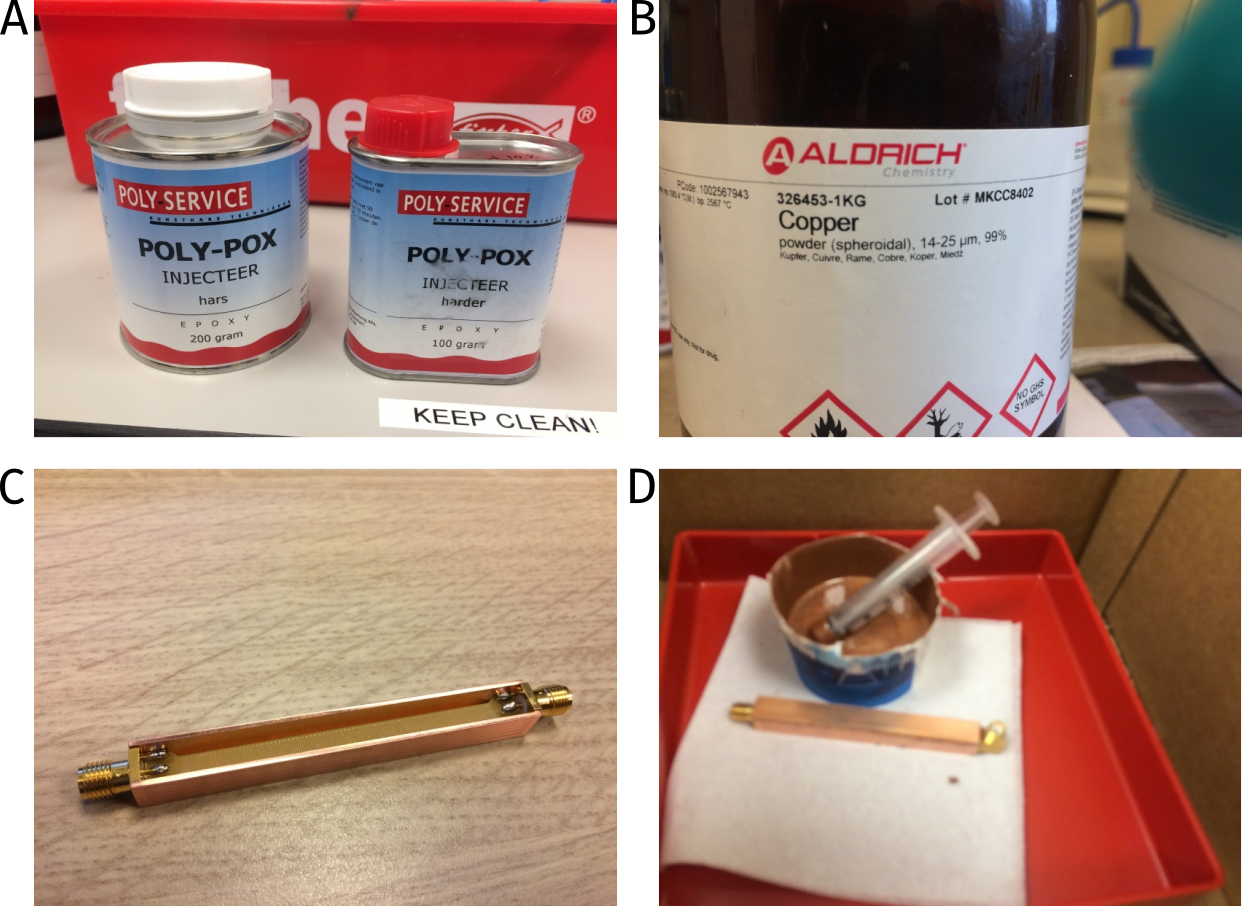
\includegraphics[]{{appendix/figs/copperpowderfilterrecipe.svg}.png}
	\caption{
		\textbf{Making copper powder filters.}
		\textbf{A,} Resin and hardener from \textit{POLY-SERVICE}.
		\textbf{B,} Copper powder from \textit{SigmaAldrich}.
		\textbf{C,} PCB with soldered SMA connectors, inside the bottom part of its copper housing.
		\textbf{D,} Dried copper powder mixture, together with a finished copper powder filter.
	}
	\label{fig:copperpowderfilterrecipe}
\end{figure}

\subsection{Instructions}
\begin{itemize}
	\item Fill \SI{10}{\gram} resin into the TUDelft coffee cup
	\item Add \SI{5}{\gram} hardener
	\item Stir for a few minutes using the spatula. The mixture should be slightly yellow and clear. Bubbles are normal. It should be very liquid.
	\item Carefully, and in the fumehood add \SI{79.5}{\gram} copper powder. The total weight should read \SI{94.5}{\gram}
	\item Stir again for a few minutes, until there are no more visible grains, also in the edges of the cup. The mixture should look like quite viscous liquid Nutella.
	\item At this point it is safe to work outside of the fume hood
	\item Cut down the walls of the coffee cup using the scissors. This will make it easier to fill the syringe
	\item Fill the syringe from the cup. One syringe should be enough for one of our usual rectangular copper boxes
	\item Slowly squirt the mixture into the copper box. Be careful, as it should go very easy! Slightly overfill the box
	\item Put the lid on and press it onto the bottom piece
	\item Using the swab, clean off mixture that got through
	\item Leave the rest of the mixture with the syringe next to the copper powder filter box for about a day
	\item Copper powder filter hardening.jpeg
	\item The next day, if the mixture inside the cup is solid, then it will also be solid inside the box because it is a chemical reaction that hardens the epoxy, not evaporation
\end{itemize}

\subsection{Testing the filter}
\begin{itemize}
	\item Measure the through resistance using a handheld multimeter. Typical through-resistance is around \SI{3}{\ohm}
	\item Measure the resistance center pin to ground, should be open
	\item Connect the filter to a VNA and measure the transmission using cryocompatible cables at RT
	\item Dunk the filter into liquid nitrogen and repeat the measurements repeatedly
	\item Note that when taking the filter back out of nitrogen, the inside might be shorted to ground because of air moisture. After one hour it should be back to normal again
\end{itemize}

\references{dissertation}

